% \documentclass[12pt]{article}

%%v helpful MIT exam schema, see http://www-math.mit.edu/~psh/exam/examdoc.pdf
 \documentclass[9pt]{exam} 
% \qformat{\textbf{Question \thequestion}\quad \thepoints\hfill } % Large depth to make space}
 \renewcommand{\thesubpart}{(\roman{subpart})}
 \renewcommand{\subpartlabel}{\thesubpart}
 \footer{}{}{}
\addpoints
\pointsinmargin
%\boxedpoints
\renewcommand{\questionshook}{\setlength{\itemsep}{2mm}}
\renewcommand{\partshook}{
	\setlength{\itemsep}{0.5cm}
%   	\setlength{\leftmargin}{-10pt}%
}

\usepackage{cmbright}

\addtolength{\jot}{2em} % this makes all formulae a bit more spaced vertically for handouts
\setlength{\parindent}{0pt} %we're not writing a novel
\renewcommand{\arraystretch}{3} %makes tables taller, so easier to write in

\usepackage[fleqn]{amsmath}
\usepackage{amssymb} %standard classy maths symbols
\usepackage[a4paper, margin=1in]{geometry} %makes it easy to specify where to put stuff on the page

\usepackage[utf8]{inputenc}

\usepackage{textcomp} % and more help for special characters

\usepackage{tcolorbox} % basic but good package for boxes around text
\tcbset{colback=black!5!white}



\usepackage{tikz} % interval diagrams, sets, etc.

\begin{document}

\textbf{Name:} \dotfill \emph{without a calculator.}

\begin{center}
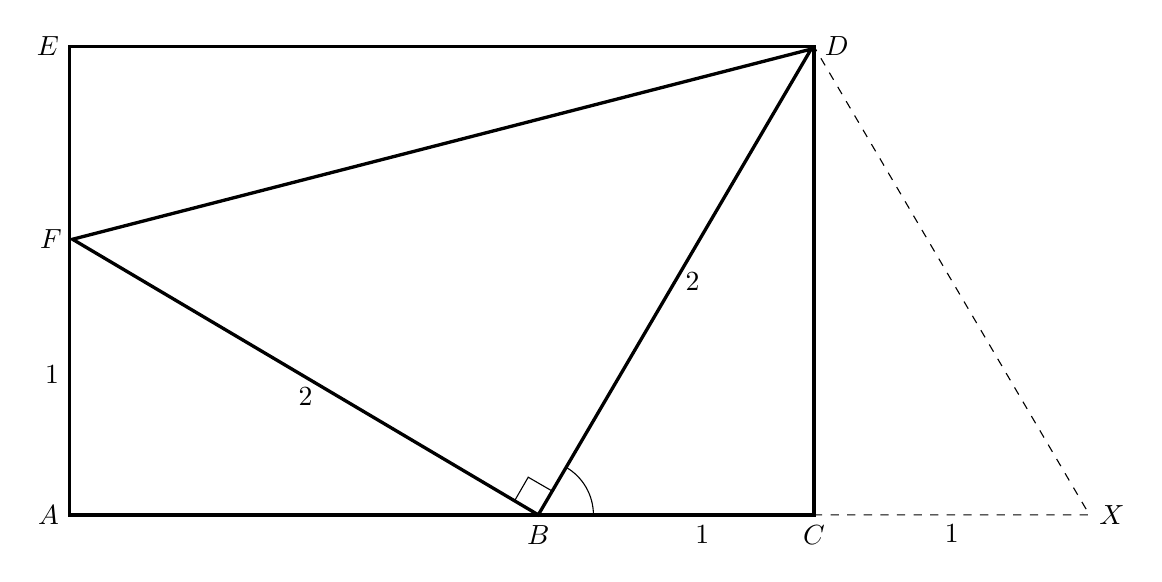
\begin{tikzpicture}[scale=3.5]

\draw[very thick] (-1.7, 0) node[left]{$A$} -- node[pos=0.85, below]{1} (1, 0) node[below]{$C$} -- (1, 1.7) node[right]{$D$} -- (-1.7, 1.7) node[left]{$E$} -- node[pos=0.7, left]{1} cycle;
\draw[very thick] (0, 0) node[below]{$B$} -- node[right]{2} (0.99, 1.69) -- (-1.69, 1) node[left]{$F$}  -- node[below]{2} cycle;
\draw[rotate around={60:(0,0)}] (0, 0) rectangle ++(0.1, 0.1);
\draw[dashed] (1,0) -- node[below] {1} (2,0) node[right] {$X$} -- (1, 1.7);
\draw (0.2, 0) arc (0:60:0.2);

\end{tikzpicture}
\end{center}


\begin{questions}

\question[2] $ACDE$ is a rectangle and $\overline{BC} = \overline{CX} = 1$. What is the nature of the triangle $\triangle BXD$? Fill in $\angle CBD$.
\fillwithdottedlines{8mm}

\question[2] What is the nature of the triangle $\triangle BDF$ ? Show this implies $\angle BDF = \angle BFD = 45^\circ$.
\fillwithdottedlines{18mm}

\question[3] Find the length $\overline{CD}$. \hfill \emph{Check hypotheses! State theorems!}

\fillwithdottedlines{27mm}

\question[6] Fill in all the angles and lengths of the diagram.

\question[2] Using $\triangle BDF$, show $\tan 45^\circ = 1$. Then use $\triangle DEF$ to find $\sin 15^\circ$ as a reduced exact value.
\fillwithdottedlines{\stretch{1}}

\question[0] \textbf{Bonus.} Fill in as much of the table of exact values overleaf as possible.

\end{questions}

\begin{tcolorbox}

\textbf{Name of marker:}

\begin{center}
\gradetable[h][questions]
\end{center}

\end{tcolorbox}

\newpage

\begin{center}
\LARGE
\begin{tabular}{|c|p{3cm}|p{3cm}|p{3cm}|}
\hline
\(\alpha\) & \(\sin \alpha\) & \(\cos \alpha\) & \(\tan \alpha\) \\
\hline
\(0^\circ\)   &               &               &               \\ \hline
\(15^\circ\)  &               &               &               \\ \hline
\(30^\circ\)  &               &               &               \\ \hline
\(45^\circ\)  &               &               &               \\ \hline
\(60^\circ\)  &               &               &               \\ \hline
\(75^\circ\)  &               &               &               \\ \hline
\(90^\circ\)  &               &               &               \\
\hline
\end{tabular}
\end{center}

\end{document}